\section{Progress}
\label{sec:progress}
%Summarise the progress you have made so far. You can cross-reference other sections (\Cref{sec:background}).
\subsection{Sourcing an FPGA}
It was quickly identified that a larger FPGA was required in order to achieve the full project aims. The current Nexys A7-100T\cite{nexys-a7-100t} has 15,850 slices, each of which contain 4 LUTs for a total of 63,400. This is inadequate, as the SoC requires 10,800 LUTs + 27,500 LUTs per "big" RV64 rocketcore, preventing more than 1 "big" RV64 rocketcore being implemented on the FPGA.

The other option for a larger core is the Sonic BOOM RV64 cores. These have a much larger LUT requirement, with the "medium" BOOM\cite{boom-core} RV64 core using 148,500 LUTs, which is clearly not possible to implement on the current FPGA.

Alternative boards are the Nexys Video and Genesys 2. The Nexys Video contains 134,600 LUTs and would allow for multiple "big" rocketcores to be implemented, but would be unlikely to fit any BOOM cores. The Genesys 2 contains 203,800 LUTs and would allow for a BOOM and "big" rocketcore to be implemented at once. Due to monetary reasons, the Nexys Video was chosen as the FPGA to be sourced. The board is currently out of stock from University sources, so no progress has been made towards purchasing it.

\subsection{SoC Design}
An initial SoC design has been created, consisting of a large and small core. This is using the rocketchip\cite{rocketchip} RV64 cores, and are generated using a Chisel description of the processor, with the large core being the "big" rocketcore and the small core the "small" rocketcore. The difference between these are changes to the instruction set extensions implemented and the size of the instruction and data caches. This change reduces the core footprint and LUT utilisation on the FPGA significantly, from an estimated 27500 LUTs to only 7600 LUTs. This is a significant reduction, though comes with the cost of reduced functionality in the smaller core.

\begin{figure}[h!]
    \centering
    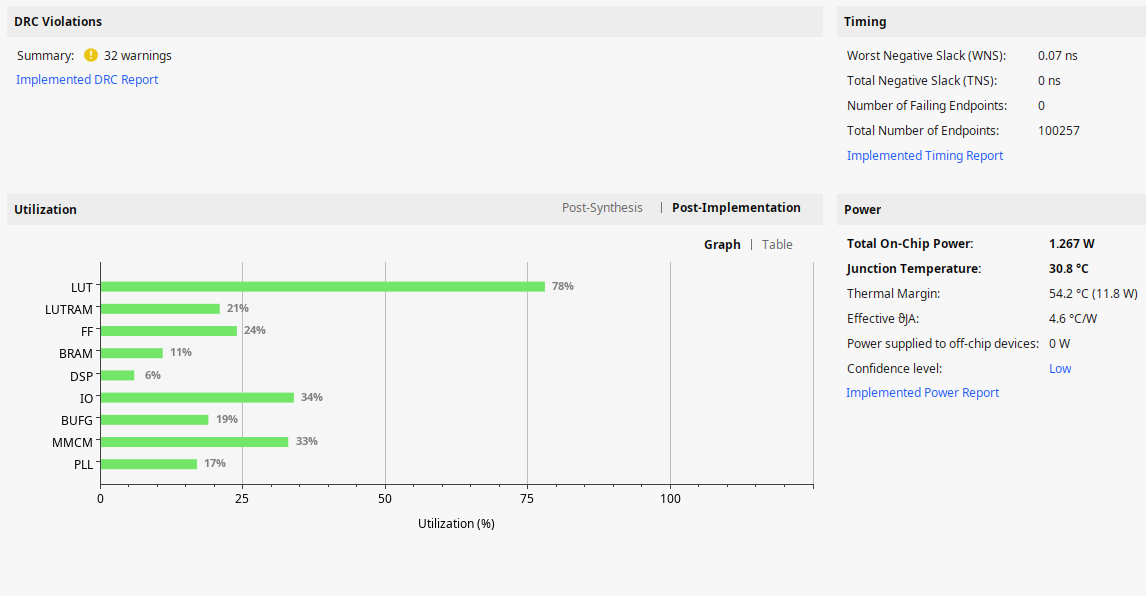
\includegraphics[scale=0.5]{./img/SoC_b1.png}
    \caption{Hardware utilisation of SoC with 1 "big" core}
    \label{fig:b1-util}
\end{figure}

\begin{figure}[h!]
    \centering
    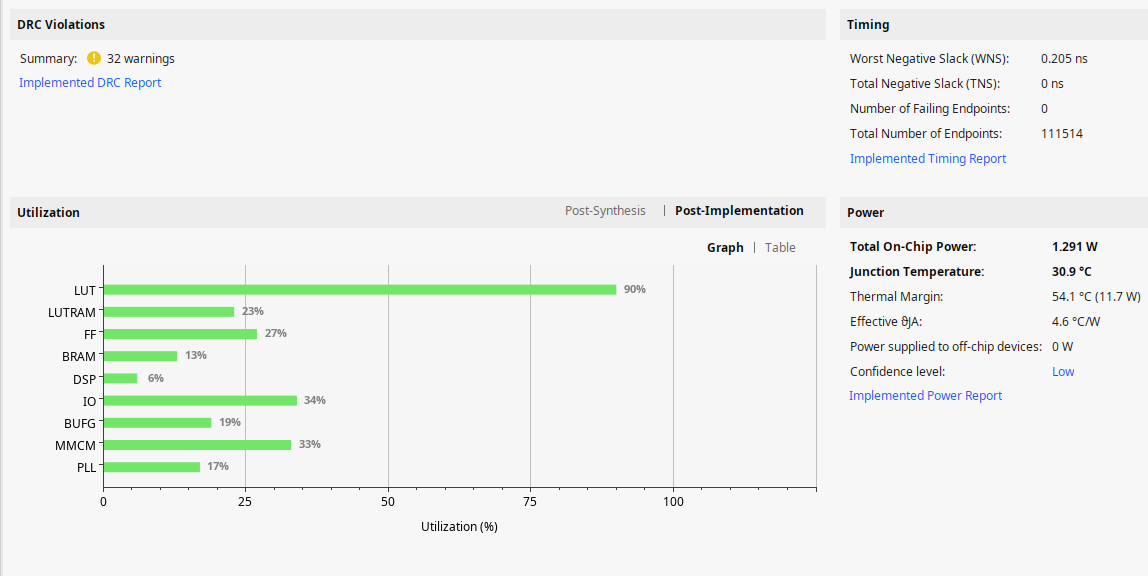
\includegraphics[scale=0.5]{./img/SoC_b1s1.png}
    \caption{Hardware utilisation of SoC with 1 "big" core and 1 "small" core}
    \label{fig:b1s1-util}
\end{figure}

\subsubsection{Core Designs}
The "big" core implements the RV64IMAFDZicsrZifenciC\cite{riscv-1} instruction set extensions. The IMAFDZicsrZifenci are commonly shortened to G, and are instructions for integer multiplication and division, atomic instructions, single-precision floating-point arithmetic, double-precision floating-point arithmetic, control and status registers and instruction-fetch fence. The final extension, C, is for compressed instructions, allowing the width of an instruction to be just 16 bits instead of the standard 32 for certain instructions. 

The "small" core reduces this to RV64IAZicsrZifenciC\cite{riscv-1}, removing multiplication and both types of floating-point arithmetic. This reduces the capability of the core significantly, and means programs compiled for the "big" core that utilise the extensions unique to the "big" core will not run on the "small" core. This does not follow the original project idea exactly, as the cores were to be equal/very similar in ability to execute instructions, but dissimilar in total processing power due to other factors like pipelining, cache, superscalar, etc. However, this has been unavoidable due to the inability to source a new FPGA in the time frame.

Currently, these cores are the standard designs included in RocketChip\cite{rocketchip}. However, there are future plans to modify the cores to be better suited to the tasks to be done on the SoC and the size of the available FPGA.

\subsection{Software}
\subsubsection{Linux}
Debian Linux was successfully run on a design implementing a single "big" RV64 rocketcore, and was used for tasks like internet messaging using IRC\cite{irc} and basic text editing. The FPGA was connected to using Minicom\cite{minicom}, a USB serial CLI tool.

IMAGINE THERES A SCREENSHOT OF A LINUX TERMINAL HERE

The "big" RV64 rocketcore is the minimum required to run mainstream Linux, as smaller designs forgo the memory-management unit (MMU). When present, the MMU is responsible for the transfer for data between the registers and memory, as well as ensuring only valid/safe memory addresses are used. When an MMU is not present, there are no checks on the memory that a program is accessing. This is a massive security issue if allowed in the OS, especially in a mainstream OS that could be attacked by malware. As such, mainstream Linux is not compatible with a processor without an MMU\cite{linux-memory} and therefore not with any processor containing a core smaller than the RV64 "big" rocketcore. As the Nexys A7 FPGA supports a single "big" rocketcore, Debian Linux\cite{debianriscv} was successfully run on an SoC design containing a single "big" rocketcore. This demonstrates that a processor containing cores equal or larger than the "big" rocketcore would be able to run mainstream linux.

The MMU requirement blocks the objective of running the RISC-V Debian Linux distribution on a custom heterogenous SoC, as the larger Nexys Video FPGA has not yet been sourced and will not be for several months. As such, the aims for software to run on the produced SoC have been reduced to bare-metal, with the stretch objective of embedded linux in the future. Embedded linux would not require an MMU\cite{linux-memory}, but would provide an extremely small amount of features when compared to Debian Linux, and have stringent constraints on the software running.

\subsubsection{Bare-metal software}
Bare-metal code has successfully been written, compiled and run on various SoC designs implemented on the FPGA. A design containing a single "big" rocketcore was implemented on the FPGA, and an SD card inserted into the board containing an ELF executable that was then run by the SoC after boot. The code outputted text over a serial connection that was then read by the host computer, and identified the 'hart' (hardware thread) of the core.

\begin{figure}[h!]
    \centering
    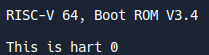
\includegraphics[scale=1]{./img/bare-metal-hart-id.png}
    \caption{Serial output of bare-metal program}
    \label{fig:bare-metal-hart}
\end{figure}

This was followed by attempting to run on the heterogeneous design previously mentioned. The only serial output received only identified a hart of 0, indicating only a single core was running the ELF executable. Investigation of the default bootrom, assembly code that sets up the core and starts the user executable, revealed that only hart's with an id of 0 started running user code - else they were trapped in a loop of waiting for an inter-processor interrupt to indicate they should execute code in a region of memory stored in a local register. The solution for this is to generate an interrupt and load the register with the location of the ELF, or to adjust the bootrom so that harts always branch to user code. In-line assembly in the C code to generate the interrupt and load the register is currently being worked on.

The current bare-metal software has all been written in C, and then cross-compiled using GCC for RISC-V. Rust is also a candidate language for bare-metal RISC-V programming\cite{rust-riscv}, and comes with certain benefits that improve usability, such as good type checking and memory safety. Changing from using C to Rust is currently being considered, and will be tested.